\chapter{Onderzoeksopzet}
\label{chap:Onderzoeksopzet}
Voor dit onderzoek wordt de methodiek van \textit{Wat is Onderzoek?} \Parencite{Verhoeven} toegepast. 
Dit hoofdstuk omvangt de ontwerpfase van het onderzoek in de onderzoekscyclus (zie figuur \ref{fig:OntwerpenCyclus}).
Eerst wordt de doelstelling van het onderzoek besproken om vervolgens een hoofdvraag te formulieren voor het onderzoek.
Daarna wordt de methodologie beschreven van het onderzoek.

\begin{graphic}
	\vspace{0.2cm}
	\captionsetup{type=figure}
    \caption{Deel 1 Verhoeven ontwerpen afgeleid van \textit{Wat is Onderzoek?}}
	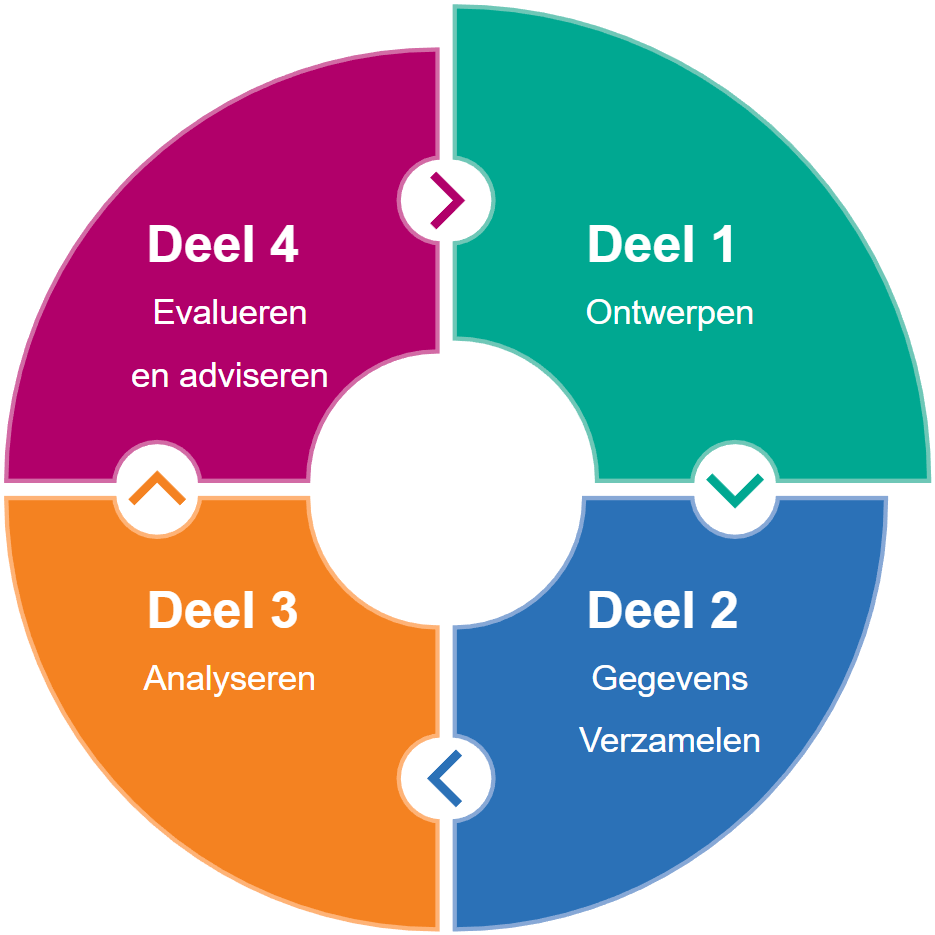
\includegraphics[scale=0.3]{img/OntwerpenCyclus.png}
	\label{fig:OntwerpenCyclus}
	\vspace{0.2cm}
\end{graphic}

\section{Doelstelling}
\label{sec:Doelstelling}
Om het proof of concept te realiseren moet er eerst bekend zijn wat er gemaakt moet worden en voor wie.
Hierom moet er een lijst aan geprioriteerde requirements komen voor 22 november 2023 voor het \qw{het CMS voor iedereen} project.
Deze lijst moet worden samengesteld in samenwerking met de stakeholders. Hierom is de volgende hoofdvraag opgesteld:

\whitespace
\begin{center}
    \textit{\MainQuestion}
\end{center}

\newpage
\section{Methodologie}
In dit hoofdstuk wordt de methodologie van het onderzoek beschreven.
Om een volledig antwoord te kunnen geven op de hoofdvraag, wordt deze vraag opgedeeld in meerdere deelvragen.
Voor het beantwoorden van de verschillende deelvragen wordt er gebruikt gemaakt van de onderzoeksmethoden die beschreven zijn door HBO-I \Parencite{HBO-i-reasearch-methods}.
% \todo[inline]{Dot framework ?}
\subsection{Deelvraag 1: Stakeholders}
Voor het opstellen van de requirements is het belangrijk om te weten voor wie het product gemaakt wordt.
Daarom is het belangrijk om de stakeholders van het project in beeld te brengen.
Hierom wordt de volgende deelvraag gesteld:

\begin{center}
	\textit{\SubquestionOne}
\end{center}

\whitespace[0.2]
Om deze deelvraag te beantwoorden wordt er een \textbf{stakeholdersanalyse} uitgevoerd.
Dit wordt gedaan door samen met de product owner een \textbf{brainstorm}sessie te houden.
Na deze sessie zullen de stakeholders geprioriteerd worden op basis van belang en invloed op het project.
Tot slot worden de stakeholders weer gegeven in een stakeholders matrix (ook wel een Mendalow matrix genoemd \Parencite{MandelowMatrix} ) om hun positie weer te geven in het project.
Het resultaat van de deelvraag zou leiden tot een lijst van geprioriteerde stakeholders die gebruikt worden om de andere deelvragen te beantwoorden.
Aan het einde van de stakeholdersanalyse worden de resultaten teruggelegd aan de product owner om de resultaten te valideren.
% \todo[inline]{Resultateren de artifacts benoemen.Mendelow matrix komt uit de lucht vallen}
% \todo[inline]{\textit{Wie is de product owner in deze context? is hij te vertrouwen om gegevens hiervoor te leveren? en waarom?}, bang dat ik te kort kom aan woorden}

\subsection{Deelvraag 2: Architectuur}
Om de huidige problemen van het Snakeware Cloud platform in beeld te brengen is het belangrijk dat er gekeken wordt naar de huidige softwarearchitectuur.
Hier uit wordt een lijst met problemen verzameld die de huidige softwarearchitectuur nu heeft.
Daarom is de volgende deelvraag opgesteld:

\begin{center}
	\textit{\SubquestionTwo}
\end{center}

\whitespace[0.2]
Door te onderzoeken hoe de huidige softwarearchitectuur in elkaar zit en onderhouden is kan er een beeld geschetst worden van de huidige problemen met Snakware Cloud.
Hierom is er voor gekozen om gebruik te maken van \textbf{IT architecture sketching} om de huidige softwarearchitectuur in beeld te brengen.
Deze onderzoekmethode wordt samen uitgevoerd met het R\&D team.
% Samen met het R\&D team zal er een sessie gepland worden om de huidige architectuur in beeld te krijgen.
Als resultaat wordt er een gesimplificeerd  domein en database model gemaakt.
Deze modellen worden gebruikt ter ondersteuning van deelvraag 3.
% Het resultaat dat uit deze deelvraag komt wordt gebruikt ter ondersteuning van deelvraag 3.
% \todo[inline]{verwachte resultaat?}

\newpage
\subsection{Deelvraag 3: Knelpunten}
Een van de doelen van het proof of concept is het oplossen van de huidige problemen die de klant en Snakeware nu hebben met het huidige systeem.
Daarom is het belangrijk om de huidige knelpunten van het systeem te inventariseren.
Hierom is de volgende deelvraag gemaakt:

\begin{center}
    \textit{\SubquestionThree}
\end{center}

\whitespace[0.2]
Om deze deelvraag te beantwoorden wordt er een semigestructureerd \textbf{expertinterview} gehouden.
Binnen Snakeware zijn er meerdere mensen die geschikt zijn om de knelpunten van het Snakeware Cloud platform te kunnen aankaarten.
Bij de volgende mensen worden de interviews afgenomen:
\begin{itemize}
    \item[-] Janny Reitsma (Service desk lead): Janny heeft veel inzicht in waar de huidige klanten van Snakeware tegen aanlopen.
        Verder krijgt ze alle klachten van de klanten van Snakeware mee en weet ze waar de huidige klanten van Snakeware behoefte aan hebben.
    \item[-] Rob Douma (Product owner van meerdere projecten): Rob werkt aan meerdere projecten als product owner en weet veel van Snakeware Cloud.
        Hij heeft veel technische kennis over het platform en kan goed in beeld brengen wat de huidige technische limitaties zijn van het platform.
\end{itemize}
%
% \whitespace
% Er is overwogen om Hans Hoomans (CEO) en Johan Nieuwehuis (CTO) te interviewen om de huidige knelpunten in beeld te brengen.
% Dit is uiteindelijk niet gedaan vanwege de tijd die beschikbaar is voor het onderzoek.
% Hierdoor mist er een stukje toekomst visie van het resultaat.

\subsection{Deelvraag 4: Requirements}
Om het systeem te kunnen ontwikkelen moeten er requirements aan het systeem gesteld worden.
Deze requirements moeten op basis van de eisen en wensen van de stakeholders gemaakt worden.
Daarom is de volgende deelvraag gemaakt:

\begin{center}
 \textit{\SubquestionFour}
\end{center}

\whitespace[0.2]
Om deze deelvraag te beantwoorden wordt er gebruik gemaakt van \textbf{explore user requirements}.
Voor de sleutelfiguren worden er semigestructureerde \textbf{interviews} gehouden om genoeg vrijheid te geven tijdens de gesprekken om dieper op vragen in te gaan.
 Voor de focus groep zal er gebruik gemaakt worden van een aantal voorbereide vragen om de focus groep in een goede richting te sturen.
Het resultaat van deze deelvraag zou leiden tot een lijst van eisen en wensen die worden vertaald in requirements.
Als de eisen en wensen zijn bepaald door middel van de interviews worden ze genoteerd zodat ze in de volgende deelvraag geprioriteerd kunnen worden.

\newpage
\subsection{Deelvraag 5: Prioritering}
Om de lijst van requirements van deelvraag 4 bruikbaar te maken moeten ze geprioriteerd worden.
% Na het opstellen van een lijst van requirements als resultaat van deelvraag 4.
% Deze lijst is echter nog niet bruikbaar, aangezien deze niet is geprioriteerd.
Om de prioriteiten van de requirements vast te stellen, wordt de volgende deelvraag geïntroduceerd.

\begin{center}
	\textit{\SubquestionFive}
\end{center}

\whitespace[0.2]
Dit wordt gedaan door middel van \textbf{requirements prioritization} er zullen verschillende prioriteit niveaus toegekend worden aan de requirements.
Deze niveaus worden in beeld gebracht door middel van MoSCoW-methode \Parencite{MoSCoW}.
Om de prioritering te bepalen wordt er gebruik gemaakt van een formule.
Deze formule en de uitleg van de deze methode is te vinden in sectie \ref{sec:Prioritering}.

% Om de prioritering te bepalen wordt er gebruik gemaakt van een formule (zie formule \ref{eq:prioritization}).
% Voor deze formule worden de volgende aspecten meegenomen:
% \begin{enumerate}
% 	\item[-] Tevredenheidsscore (TS) [1,2,\ldots,5]: dit is de waarde die door de stakeholder gegeven wordt als de requirement geïntroduceerd wordt.
% 	      Waarbij een hoge waard ede tevredenheid aangeeft als het geïntroduceerd wordt.
% 	\item[-] Ontevredenheidscore (OS) [1,2,\dots,5]: Dit is de waarde die door de stakeholder gegeven wordt wanneer het niet geïntroduceerd wordt.
% 	      Waarbij de hoge waarde de ontevredenheid aangeeft als het niet geïntroduceerd wordt.
% 	% \item[-] Stakeholder invloed positie (SIP) [1,2,3,4]: Op basis van de stakeholders matrix wordt er een waarde aan een stakeholder groep toegekend 4 voor sleutelfiguren, 3 voor beinvloeder, 2 voor geïnteresseerde en 1 voor toeschouwer.
% 	\item[-] Duur [1,2,3,5,8]:
%         De duur wordt gerepresenteerd om een grove schatting te geven van de realisatie tijd van de requirement.
% 	    De waardes van de duur zijn een verkleinde selectie van Scrum poker \Parencite{ScrumPoker}.
% \end{enumerate}
%
% \whitespace
% \begin{equation}
% 	\label{eq:prioritization}
% 	Score = TS + OS + (9 - duur)
% \end{equation}
%
% \whitespace
% Nadat er een score is berekend wordt er een prioriteit niveau toegewezen op basis van de MoSCoW-methode.
% De waardes van de prioriteiten zijn toegekend en gevalideerd door de product owner:
%
% \whitespace
% \makebox[3cm][l]{Must have:} $ x \in \mathbb{R} : 14 \leq x \leq 18 $ \\
% \makebox[3cm][l]{Should have:} $ x \in \mathbb{R} : 9 \leq x \leq 13 $ \\
% \makebox[3cm][l]{Could have:} $ x \in \mathbb{R} :  5 \leq x \leq 8 $ \\
% \makebox[3cm][l]{Won't have:} $ x \in \mathbb{R} : 3 \leq x \leq 4 $
%
\whitespace
Als de requirements geprioriteerd zijn worden ze genoteerd in verschillende user stories.
Bij de user story staat het Id van de requirement aangegeven zodat het makkelijk te identificeren is.
De prioriteit wordt aangegeven door de verschillende MoSCoW prioriteit niveaus
% Daarnaast wordt de duur aangegeven met de duur waarde die gebruikt is in de formule.
In tabel \ref{rq:TMP1} is een voorbeeld van een user story te zien.
Na het maken van de user stories wordt er terug gekoppeld naar de stakeholders om het resultaat te verifiëren.
Als de volledige lijst gemaakt is wordt de lijst gecheckt door de product owner en de bedrijfsbegeleider.

% \todo[inline]{Fix formule met naam er bij}
% \todo[inline]{Leg schaal 1 tot 5 uit}
\Requirement{TMP1}{Must have}{3}{Dit is een test user story}{Dit zijn de acceptatiecriteria}

% \todo[inline]{Scores zijn nu tijdelijk is nog geen moment om dit te valideren met de product owner en is ook pas handig dat gedaan wordt als de stories gemaakt zijn}


% \section{Onderzoeksvragen}
Om de doelstelling van het onderzoek te behalen moeten de stakeholders geïdentificeerd worden.
Door middel van de stakeholders kan er een lijst van requirements opgesteld worden.
Hierom is de volgende hoofdvraag opgesteld.

\whitespace
\textit{\textbf{Hoofdvraag:} \MainQuestion}

\whitespace
Om een volledig antwoord te kunnen geven op de hoofdvraag, wordt deze vraag opgedeeld in meerdere deelvragen.
Elke van deze deelvragen wordt afzonderlijk behandeld om een omvattend antwoord te krijgen.

\whitespace
Voor het opstellen van de requirements is het belangrijk om te weten voor wie je het maakt.
Daarom is het belangrijk om de stakeholders van het project in beeld te brengen. 
Hierom is de volgende deelvraag gebruikt:

\whitespace
\textit{\textbf{Deelvraag 1:} \SubquestionOne}

\whitespace
Om de huidige problemen van het Snakeware cloud platform in beeld te brengen is het belangrijk dat er gekeken wordt naar de huidige software-architectuur.
Hier uit wordt een lijst met problemen verzameld die de huidige software-architectuur nu heeft, en wordt ter ondersteuning gebruikt voor deelvraag 3 (\textit{\SubquestionThree}).
Daarom is de volgende deelvraag opgesteld:

\whitespace
\textit{\textbf{Deelvraag 2:} \SubquestionTwo}

\whitespace
Omdat een van de doelen van het  proof of concept is het oplossen van de huidige problemen die de klant en Snakeware heeft met het huidige systeem.
Daarom is het belangrijk om te inventariseren wat de huidige knelpunten zijn van het systeem. 
Hierom is de volgende deelvraag gemaakt:

\whitespace
\textit{\textbf{Deelvraag 3:} \SubquestionThree}

\whitespace
Om het systeem te kunnen ontwikkelen moeten er requirements aan het systeem gesteld worden.
Deze requirements moeten op basis van de eisen en wensen van de stakeholders gemaakt worden.
Hier uit zal een lijst requirements komen waar mee het systeem gerealiseerd wordt.
Daarom is de volgende deelvraag gemaakt:

\whitespace
\textit{\textbf{Deelvraag 4:} \SubquestionFour}

\whitespace
Nadat er een lijst van requirements zijn opgesteld als resultaat van deelvraag 3.
Deze lijst is nog niet handig om te gebruiken omdat de lijst niet geprioriteerd is.
Om deze lijst te prioriteteren wordt de volgende deelvraag gesteld.

\whitespace
\textit{\textbf{Deelvraag 5:} \SubquestionFive} \\

% \newpage
% \section{Onderzoeksmethoden}
In dit hoofdstuk zal er worden toegelicht welke onderzoeksmethode gekozen is voor elke deelvraag met daar bij een onderbouwing.
Om de validiteit van het onderzoek te waarborgen is er gebruik gemaakt van \textit{ICT-research methods} \Parencite{HBO-i-reasearch-methods}.

\whitespace
\textit{\textbf{Deelvraag 1:} \SubquestionOne}

\whitespace
Om deze deelvraag te beantwoorden wordt er een \textbf{stakeholdersanalyse} uitgevoerd.
Dit wordt gedaan door samen met de product owner een \textbf{brainstorm} sessie te houden.
Na deze sessie zullen de stakeholders geprioriteerd worden op basis van belang en invloed op het project.
Tot slot worden de stakeholders in een Mendelow matrix \Parencite{MandelowMatrix} geplaatst om hun positie weer te geven in het project.
Aan het einde van de stakeholdersanalyse worden de resultaten terug gelegt aan de product owner om de resultaten te valideren.

\whitespace
\textit{\textbf{Deelvraag 2:} \SubquestionTwo}

\whitespace
Door te onderzoeken hoe de huidige software architectuur in elkaar zit en onderhouden is kan er een beeld geschetst worden van de huidige problemen met Snakware Cloud.
Hierom is er voor gekozen om gebruik te maken van \textbf{IT architecure sketching} om de huidige softwarearchitectuur in beeld te brengen.
Samen met het R\&D team zal er een sessie gepland worden om de huidige architectuur in beeld te krijgen.
Het resultaat dat uit deze deelvraag komt wordt gebruikt ter ondersteuning van deelvraag 3.

\whitespace
\textit{\textbf{Deelvraag 3:} \SubquestionThree}

\whitespace
Om deze deelvraag te beantwoorden wordt er een semi-gestructureerde \textbf{expert interview} gehouden met X-X om er achter te komen wat de huidige knelpunten zijn bij Snakeware cloud.
Na de expert interviews zal er een \textbf{task analyse} uitgevoerd worden om de werkwijze (workflows) in beeld te krijgen.

\todo[inline]{met wie is het beste om het interview te houden janny, hans of johan of allemaal (ben dan alleen bang voor tijd)}
\todo[inline]{ook te kort denk ik}

\whitespace
\textit{\textbf{Deelvraag 4:} \SubquestionFour}

\whitespace
Om deze deelvraag te beantwoorden wordt er gebruik gemaakt van \textbf{explore user requirements}.
De communicatie methode met de stakeholders wordt bepaald op basis van hun positie binnen het project door middel van de Mandelow matrix.
Voor de sleutelfiguren worden er semigestructureerde \textbf{interviews} gehouden om genoeg vrijheid te geven tijdens de gesprekken om dieper op vragen in te gaan.
Daarnaast worden er met de geïnteresseerde een \textbf{Focus group} gepland om hier met de betrekende stakeholders meerdere onderwerpen te bespreken die belangrijk zijn voor het project.
Voor de focus groep zal er gebruik gemaakt worden van een aantal voorbereide vragen om de focus groep in een goede richting te sturen.
Als de eisen en wensen zijn bepaald door middel van de focus group en interviews worden ze genoteerd zodat ze in de volgende deelvraag geprioriteerd kunnen worden.

\whitespace
\textit{\textbf{Deelvraag 5:} \SubquestionFive}

\whitespace
De lijst van requirements uit deelvraag 4 moet nog worden verwerkt om er gebruikt van te kunnen maken.
Dit wordt gedaan door middel van \textbf{requirements prioritization} zal er verschillende prioriteit niveaus toegekend worden aan de requirements.
Deze niveaus worden in beeld gebracht door middel van MoSCoW-methode \Parencite{MoSCoW}.

De prioriteit van de requirements wordt berekend op basis van de invloed en het belang van de stakeholders,
de tevredenheidsscore [1,2,\ldots,5] bij implementatie, de ontevredenheid score [1,2,\ldots,5] als het niet geïmplementeerd wordt en de duur van de implementatie (1,2,3,5,8) die wordt weer gegeven door een relatief getal.
De berekening wordt gedaan door middel van de volgende formule:

\whitespace
\begin{center}
	\(Score = tevredenheidsscore - ontevredenheid score + (9 - duur)\)
\end{center}

\whitespace
nadat er een score is berekend wordt er een prioriteit niveau toegegeven op basis van de MoSCoW methode:

\whitespace
Must have:  \(x \in \mathbb{R} : 14 \leq x \leq 18\)

\whitespace
Should have: \(x \in \mathbb{R} : 14 \leq x \leq 18\)

\whitespace
Could have: \(x \in \mathbb{R} : 14 \leq x \leq 18\)

\whitespace
Won't have: \(x \in \mathbb{R} : 14 \leq x \leq 18\)

\whitespace
De requirement worden vervolgens genoteerd in een gemodificeerde versie van een snow card.
Na het maken van de requirement wordt er terug gekoppeld met de stakeholder om het te verifiëren
als de volledige lijst gemaakt is wordt het gecheckt met de product owner en de bedrijfsbegeleider.

\todo[inline]{Maak fancy snow card en fancy formule en daarna tekst verbeteren scores kloppen ook nog niet want deze moeten besproken worden en eigelijk pas gesteld worden tijden de deelvraag ?}

